\documentclass[a4paper,10pt]{article}
\usepackage[margin=3cm, nohead]{geometry}
\usepackage{natbib}
\usepackage{graphicx}
\usepackage{algorithmic}

\newcommand{\HRule}{\rule{\linewidth}{0.5mm}}

\begin{document}

\begin{titlepage}
\begin{center}

\includegraphics[width=1\textwidth]{uva}\\[1cm]

\HRule \\[0.4cm]
{ \huge \bfseries Tweedejaarsproject A.E.S.I.}\\[0.4cm]

\HRule \\[1cm]

\textsc{\LARGE  Artificial Evolution and Swarm Intelligence}\\[0.5cm]
\textsc{\Large  Werkplan}\\[1cm]

\begin{tabular*}{0.95\textwidth}{@{\extracolsep{\fill}} l c r}
Jeroen \textsc{Rooijmans}	& Maarten \textsc{Inja}     & Maarten \textsc{de Waard} \\
\textsc{5887410}                &\textsc{5872464}           &\textsc{5894883}\\
\end{tabular*}

\vfill \today
\end{center}
\end{titlepage}
\tableofcontents \pagebreak

\section{Introduction}
During this project we will attempt to create a program that artificially evolves tank like agents in the RoboCode environment\footnote{RoboCode home page: http://robocode.sourceforge.net/}.
RoboCode is a simple game, where virtual tanks can fight eachother. More information and rules of the game can be found in section \ref{bi}.

It would be fairly easy to write a powerful bot ourselves, but using genetic programming\footnote{Genetic Programming wiki: http://en.wikipedia.org/wiki/Genetic\_programming} we can let a computer evolve these bots.
To test our evolved bots, we use the RoboCode environment to generate test data of battles between our evolved bots and various enemy bots. After a certain amount of battles, RoboCode generates results, these results consist of a overall score. The score is calculated using the survival rate, damage done and ranking of the previously fought battles.

There also is a tool we use, called RoboResearch\footnote{RoboResearch home page: http://robowiki.net/wiki/RoboResearch}. This tool gives bots a score in a similar way the RoboCode environment does, but uses default bots as enemies.
We use similar program that evolves RoboCode bots created by Klaus Meffert, the program is called RoboCode with JGAP\footnote{RoboCode with JGAP home page: http://jgap.sourceforge.net/doc/robocode/robocode.html}. We can use this program to generate enemy bots.

Other enemies can be bots that won online tournaments, informations and rankings of these tournaments can be found on RoboRumble\footnote{RoboRumble home page: http://robowiki.net/wiki/RoboRumble}.
The code for this project will be written in Java and available on our Google Code page \footnote{Google Code page: http://code.google.com/p/aesi/}.
We planned our activities with the Gantt chart that can be found in Appendix \ref{planning}.

When we are done evolving the single bots, we will try to adapt our program to evolve a team of bots. These will be evolved and tested the same way as the single bots.

\section{Project goals}
The main goal of this project is to create a Java program that evolves RoboCode bots.
These bots will evolve based on their performance, this performance needs to be tested. We use the results of multiple battles, acquired by the benchmark tool in RoboCode environment to give a bot a certain ``fitness'' score.
The evolution is done by manipulating the genotype of the bots. Therefor we need to create a representation that can manipulate the genotype and translate it to the phenotype.

\section{Method}
In order to evolve a powerfull agent using genetic programming, we first need to understand the underlying principles. This implies research on two subjects, powerful behavior in RoboCode and genetic programming.

Powerful behavior is documentated on RoboRumble, information about how to design our genetic algoritm is found in the article ``Evolving 3D Morphology and Behavior by Competition''\cite{karlsims}.
After acquiring enough information, we will start implementing the genetic algorithm, this will be done using the JGAP framework\footnote{JPAG home page: http://jgap.sourceforge.net/}.

\subsection{Genome}
We have to plan and create the genome of our bots. Each chromosome represents a potential solution (strong behavior) and is divided into several genes, these genes represent various aspects of the bot (shooting, moving, ect).

These ``chromosomes'' result in a Java file consisting of several methods, for example robotScannedEvent and robotHitWallEvent. These methods can make calls to various functions such as rotateGun. There are countless of different variations that can be disabled, modified or enabled by reproduction, crossover and mutations.

\subsection{Phenome}
The phenome is the resulting behaviour of the bot. This behaviour will be tested and a bot is given a certain fitness score. This is explained in ``Fitness function''. Bots with a higher fitness score, meaning it has more powerful behaviour, have a better chance to pass on their genome to the next generation.

\subsection{Meta language}
We need to design a meta language that translates a genetic code, consisting of a string of digits, to the behavior of the bot. This means the result of translation is Java code. We have to find an appropriate representation that gives the evolutionary process enough room to evolve without forcing it in a certain direction. We hope this leads to interesting and original behaviour.

\subsection{Fitness function}
When dealing with evolution, there has to be a process that favors stronger genotypes. We do this by defining a fitness function. This function evaluates every chromosome and defines a fitness, which indicates how well it performs.
We use the benchmark in the RoboCode environment, that calculates an overall score based on the performance in previously fought battles. By taking the survival rate, damage done and ranking of the previously fought battles in consideration, we will create a function that evaluates every bot and gives them a relative fitness score.

But to simulate these battles, we have to generate Java code, therefore we have to compile the code which consumes a lot of time. Creating a very elaborate fitness function will increase the time-costs, a very constrained one will decrease both time and accuracy, so we will have to find a balance to strike the golden mean.

\subsection{Evolve}
The evolutionary processes are done by the JGAP framework. Genes with a stronger fitness value have a better chance of being selected for next generations. The selected genes will be written into the Java code and the process repeats itself until either a certain amount of generations have evolved or a certain predefined fitness value is achieved.
We start our evolution with blank bot, the bot genome will consist of alot of functions, but these will need to be activated, or manipulated to actually work and therefor needs to be manipulated by the evolutionary process. The genome is manipulated by three processes: sexual reproduction, crossover, and mutation.

RoboCode with JGAP uses one bot to test a new genetion of bots, in ``Evolving 3D Morphology and Behavior by Competition``\cite{karlsims} some alternatives are explained. We will implement a ``all vs. best'' strategy. This means the bots from a new generation fight the fittest bot of the previous generation.

\section{Background information}
\label{bi}
\subsection{RoboCode Game}
Time is represented in ticks. There are several things happening each tick. For example the robot is allowed a certain amount of processing time to calculate and execute actions. The game world is also updated, meaning that objects are relocated according to the physical laws of the game and potential collisions between objects and the results of such collisions are calculated.

\subsection{Robot Anatomy}
A robot consists of three seperate parts, the radar which is mounted on the barrel which is mounted on the body. All parts can be rotated seperately. The barrel fires bullets, the radar scans for other tanks and the body drives around in the arena. 

\subsection{Robocode rules}
The Robocode environment has specific rules constraining our bot. I will explain the basic rules of the RoboCode game and how a bot can behave.
A fight starts by placing all participating bots in the arena at random places. All bots have a certain amount of energy. Energy is lost by getting shot by an enemy or ramming walls and enemies. Certain actions also use up energy, for example shooting a bullet.
A bot can gain energy by hitting an opponent.

When a bot is out of energy, it is disabled and explodes.

\subsection{Programming the Robot}
Programming a robot means \textit{extending} the robot class from RoboCode. This allows us to program methods that catch events that are launched by RoboCode (such as \textit{robotScannedEvent}) and program what we would like the robot to do in such cases (such as \textit{rotateGun}). The robots behavior relies completely on what events occur during a battle. The robots actions during a certain event is generated by the evolutionary process. 


   
    
\newpage
\section{Planning}
\subsection{Documentation}
\begin{itemize}
 \item create workplan, everybody
 \item round of halfway report and presentation, M. de Waard
 \item present halfway presentation, everybody
 \item finish end report and presentation, J. Rooijmans
 \item present final product, everybody
 \item maintain documentation, M. Inja
\end{itemize}

\subsection{Initiation}
\begin{itemize}
\item create planning and set up websites, M. Inja
\item present workplan, everybody
\item familarization with programs, M. Inja, M. de Waard
\item read articles about genetic algoritms, J. Rooijmans
\end{itemize}

\subsection{Genetic programming, single bots}
\begin{itemize}
\item create genotype, J. Rooijmans
\item create fitness function, M. de Waard
\item evolve, M. Inja
\end{itemize}

\subsection{Test phase}
\begin{itemize}
\item benchmark with RoboResearch, M. de Waard
\item compare RoboCode with JPAG, M. Inja
\item design and compare with own bot, everybody
\item compare with bots from the internet, J. Rooijmans
\end{itemize}


\subsection{Genetic programming, teams}
\begin{itemize}
\item create genotype, J. Rooijmans
\item create fitness function, M. de Waard
\item evolve, M. Inja
\item benchmark, everybody
\end{itemize}
\newpage
\bibliographystyle{agsm}
\bibliography{ref}
\newpage
\appendix
\section{Planning}
\label{planning}
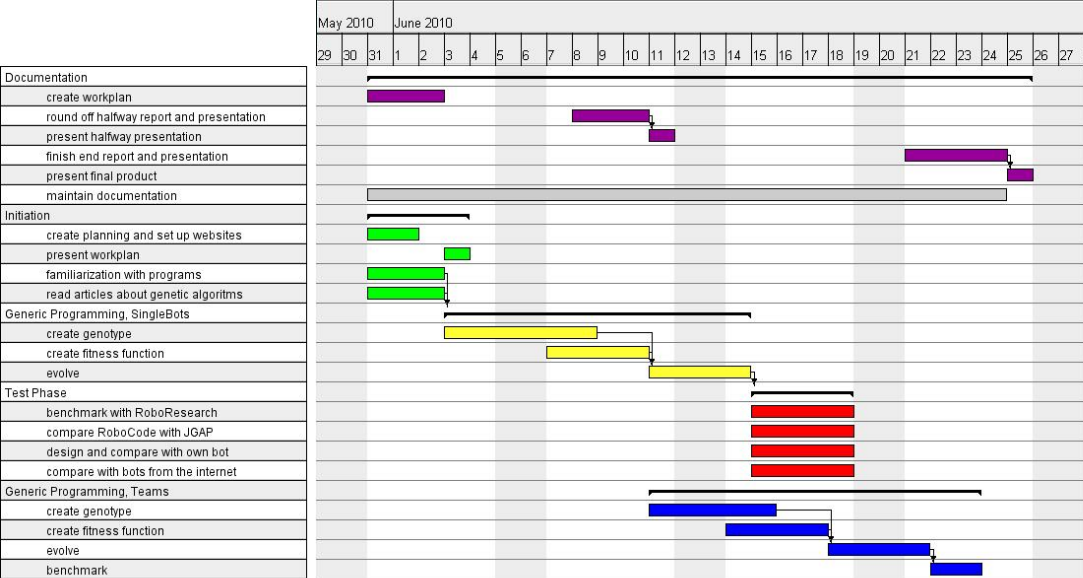
\includegraphics[height=0.75\textwidth, angle=-90]{planning.png}


\end{document}
